\documentclass[11pt]{article}
\usepackage[margin=1in]{geometry}

% Packages we need
\usepackage{amsmath}
\usepackage{mathtools}
\usepackage{amsthm}
\usepackage{float}
\usepackage{graphicx}
\usepackage{listings}
\usepackage{color} %red, green, blue, yellow, cyan, magenta, black, white

% Header packages
\usepackage{fancyhdr}
\fancyhf{}
\pagestyle{fancy}

% Algorithms
\usepackage{algorithmic}
\usepackage{algorithm}

% Formatting document
\setcounter{secnumdepth}{0}
\setlength{\parindent}{0in}
\setlength{\parskip}{0.5em}

% MATLAB code
\definecolor{mygreen}{RGB}{28,172,0} % color values Red, Green, Blue
\definecolor{mylilas}{RGB}{170,55,241}
\lstset{language=Matlab,%
    %basicstyle=\color{red},
    breaklines=true,%
    morekeywords={matlab2tikz},
    keywordstyle=\color{blue},%
    morekeywords=[2]{1}, keywordstyle=[2]{\color{black}},
    identifierstyle=\color{black},%
    stringstyle=\color{mylilas},
    commentstyle=\color{mygreen},%
    showstringspaces=false,%without this there will be a symbol in the places where there is a space
    numbers=left,%
    numberstyle={\tiny \color{black}},% size of the numbers
    numbersep=9pt, % this defines how far the numbers are from the text
    emph=[1]{for,end,break},emphstyle=[1]\color{red}, %some words to emphasise
}

% Commands
\DeclarePairedDelimiter\ceil{\lceil}{\rceil}
\DeclarePairedDelimiter\floor{\lfloor}{\rfloor}
\newcommand{\ws}{\text{ }}
\newcommand{\e}[1]{\times 10^{#1}}

% Header
\lhead{\textsc{CS 5220 -- Sep. 01 Preclass Questions}} % TODO: enter title here
\rhead{\textsc{Eric Gao -- emg222}} % Authors
\setlength{\headheight}{0.5in}
\cfoot{\thepage}

% Title
\title{CS 5220 -- Sep. 01 Preclass Questions} %TODO: enter title here
\author{
  \begin{tabular}{l c l}
    Eric Gao & -- & emg222\\
  \end{tabular}\\
  \rule{\linewidth}{0.4pt}
}
\date{}


\begin{document}
    \thispagestyle{empty}
    \maketitle

    \section*{Question 1}
        We have 60 cores per accelerator and 15 Xeon Phi accelerator boards. Each core on the Xeon Phi board has a clock speed of 1.053 GHz (http://ark.intel.com/products/71992/Intel-Xeon-Phi-Coprocessor-5110P-8GB-1\_053-GHz-60-core). These accelerators use the IMCI instruction set, which can perform 2 FLOPs per FMA and have 512 bits per instruction, which means we can perform 8 double-precision FMAs per Vector FMA, and we can perform 1 Vector FMA per cycle, since we only have 1 thread per core. The theoretical peak FLOP rate for just the accelerator boards is then:
        \begin{align*}
            15 \text{ accelerators} &\times 60 \frac{ \text{cores} }{ \text{acclerator} } \times 1.053\times 10^9 \frac{ \text{cycles} }{ \text{second core} } \\[0.5em]
                                    &\times 1 \frac{ \text{Vector FMAs} }{\text{cycle} }  \times 8 \frac{ \text{FMAs}}{\text{Vector FMA}}\\[0.5em]
                                    &\times 2 \frac{\text{FLOPs}}{\text{FMA}} = 15.16 \text{ TFLOP/s}
        \end{align*}

        We then also have 8 nodes, with 12 cores per node. Any core on these 8 nodes has a theoretical maximum clock rate of 3.5 GHz (http://ark.intel.com/products/75283/Intel-Xeon-Processor-E5-2697-v2-30M-Cache-2\_70-GHz). These processors use the SIMD (AVX) instruction set, which can perform 2 FLOPs per FMA and have 256 bits per instruction, which means we can perform 4 double-precision FMAs per Vector FMA. In addition, we have 2 threads per core, which means we can perform 2 Vector FMAs per core. Assuming these specs, the FLOP rate of our 8 compute nodes is given by:
        \begin{align*}
            8 \text{ nodes} &\times 12 \frac{\text{cores}}{\text{node}} \times 3.5\times 10^9 \frac{\text{cycles}}{\text{second core}}\\[0.5em] 
                            &\times 2 \frac{ \text{Vector FMAs} }{\text{cycle} }  \times 4 \frac{ \text{FMAs}}{\text{Vector FMA}}\\[0.5em]
                            &\times 2 \frac{\text{FLOPs}}{\text{FMA}} = 5.38 \text{ TFLOP/s}
        \end{align*}

        This gives us a total and theoretical maximum FLOP rate of: $15.16 + 5.38 = 20.54 \text{ TFLOPs}$, or about 20.5 TeraFLOPs per second.

    \section*{Question 2}
        My machine has a Haswell Intel Core i7-4770K (http://ark.intel.com/products/75123/Intel-Core-i7-4770K-Processor-8M-Cache-up-to-3\_90-GHz). There are 4 cores. It uses a SIMD (AVX) architecture, which uses 256 bit instructions, resulting in at most 4 double-precision FMAs per Vector FMA. We have 2 threads per core, so we can perform 2 Vector FMAs per core. Assuming these specs, we get a peak FLOP rate of:
        \begin{align*}
            4 \text{ cores} &\times 3.9\times 10^9 \frac{\text{cycles}}{\text{second core}} \times 2 \frac{ \text{Vector FMAs} }{\text{cycle} }\\[0.5em]
                            &\times 4 \frac{ \text{FMAs}}{\text{Vector FMA}} \times 2 \frac{\text{FLOPs}}{\text{FMA}} = 249.6 \text{ GFLOP/s}
        \end{align*}

    \section*{Question 3}
        Speedup is found by:
        \begin{equation*}
            S(p, t) = \frac{\text{Pipelined time}}{\text{Serial time}}
        \end{equation*}

        Assuming we have $t$ tasks that take $\tau$ time each, we know that the serial time is $t\tau$.

        We have a pipeline with $p$ stages, assuming we don't have any branching and don't have to flush the pipeline at any point. We also assume that each stage in the pipeline takes an equivalent amount of time. That is if a task takes $\tau$ time to complete in the pipeline, then each stage in the pipeline takes $\frac{\tau}{p}$ time if there are $p$ stages in the pipeline. Therefore, after we finish the first task in $\tau$ time, we finish the each of the remaining tasks in $\frac{\tau}{p}$ time. Our pipelined speed is then:
        \begin{equation*}
            time_{pipelined} = \tau + (t - 1)\frac{\tau}{p} = \tau\left(1 + \frac{t - 1}{p}\right)
        \end{equation*}

        Our speedup is then given by:
        \begin{equation*}
            S(p ,t) = \frac{1 + \frac{t - 1}{p}}{t}
        \end{equation*}

    \section*{Question 4}
        The minimum serial time, assuming no pipelining, is just the sum of the times:
        \begin{equation*}
            time_{serial} = 1 + 0.5 + 0.25 + 0.5 + 0.5 = 2.75 \text{ hr}
        \end{equation*}

        The minimum parallel time can be seen in the following table.
        \begin{table}[H]
            \centering
            \begin{tabular}{| c | c | c | c | c | c | c | c | }
            \hline
            time & 0 hr & 1 hr & 1.25 hr & 1.5 hr & 1.75 hr & 2 hr & 2.25 hr \\
            \hline \hline
                 & GCC  & GCC done & & & & & \\
            \hline
                 &      & MPI & MPI & MPI done & & &  \\
            \hline
                 &      & BLAS & BLAS done & & & & \\
            \hline
                 &      &          & LAPACK & LAPACK & LAPACK done  & & \\
            \hline
                 &      &          &        &        & App & App & App done\\
            \hline
            \end{tabular}
        \end{table}

        The minimum parallel time is therefore 2.25 hrs.

    \section*{Question 5}
        \begin{figure}[H]
            \centering
            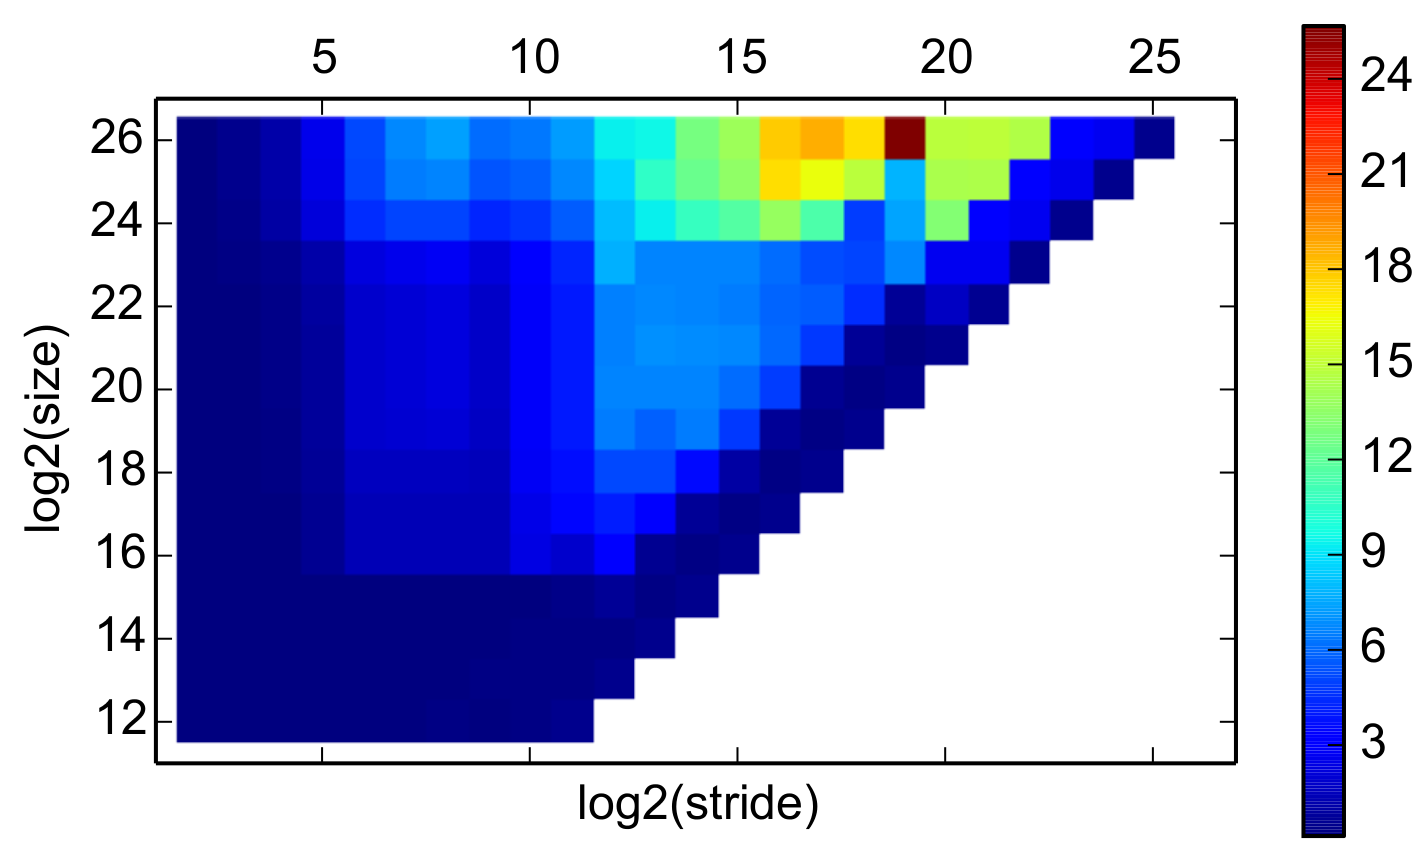
\includegraphics[width=5in]{timings/timings-heat.png}
        \end{figure}

        We first notice that membench runs extremely quickly for any array with size less than or equal to $2^{15}$ bits. This indicates that perhaps the L1 cache is 32 KB large. We then get even larger increases in time when the size of the array increases above approximately $2^{17}$ or $2^{18}$ bits, or 128 KB or 256 KB. This indicates that the L2 cache may be around 256 KB large. The final large increase in time occurs when we try to load an array of size $2^{24}$ bits or 16 MB, indicating that the L3 cache may be around 8 MB large.

        We also notice that no matter the size of the array, we have good times when the stride is small, indicating that spatial locality improves times. Similarly, we have good times when the stride is large relative to the size the array. But this might be mainly because we have to perform fewer lookups since the stride is so large.

    \section*{Question 6}
        \begin{figure}[H]
            \centering
            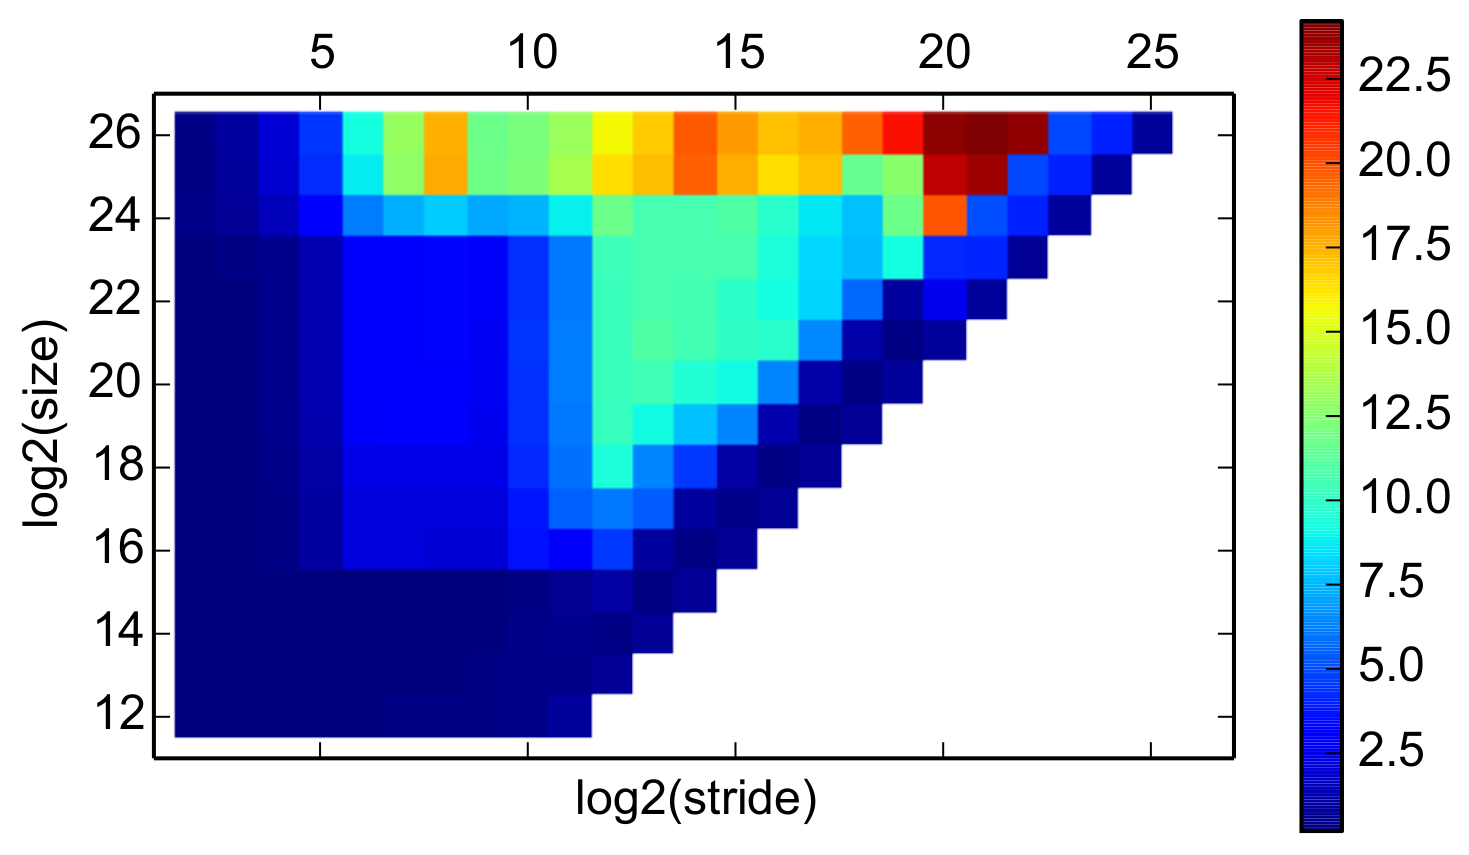
\includegraphics[width=5in]{timings-totient/timings-heat.png}
        \end{figure}

        Again we notice that membench runs extremely quickly for any array with size less than or equal to $2^{15}$ bits or 32 KB. So we can assume that the L1 cache may be roughly 32 KB large. Any size larger than $2^{18}$, we get an increase in time, indicating that the L2 cache may be either 128 KB or 256 KB large. Finally, we get another increase in time when we have an array larger than $2^{23}$, indicating that the L3 cache maybe about 8 MB large. We notice a similar pattern when compared to the previous heat map with regards to stride size.

    \section*{Question 7}
        Based on the code I wrote, the first method was the fastest, most likely because of spatial locality. The third method was the second fastest and the second method was the slowest. This was run on my local machine.

\end{document}